\setchapterpreamble[u]{\margintoc}
\chapter{Unplugging Skynet}
\labch{skynet}

\textit{"The second requirement of goal-misalignment risk is that an intelligent machine can commandeer the Earth's resources to pursue its goals, or in other ways prevent us from stopping it... We have similar concerns with humans. This is why no single person or entity can control the entire internet and why we require multiple people to launch a nuclear missile. Intelligent machines will not develop misaligned goals unless we go to great lengths to endow them with that ability. Even if they did, no machine can commandeer the world's resources unless we let it. We don't let a single human, or even a small number of humans, control the world's resources. We need to be similarly careful with machines." - Jeff Hawkins, 2022 \cite{hawkins2022}}

\section{Landmines Everywhere}

As we explore the potential of artificial intelligence in the realm of warfare, it is crucial to approach the topic of autonomous weapons with a healthy dose of skepticism. To fully grasp the inherent risks of these weapons, we need look no further than the history of landmines. These indiscriminate, uncontrollable devices should serve as a stark reminder of the potential pitfalls associated with the development and deployment of autonomous weaponry.

Landmines have long been a staple of military strategy, yet their consequences continue to plague countless communities around the world. Once deployed, landmines cannot differentiate between friend or foe, soldier or civilian. They lie dormant, waiting to unleash their destructive force on unsuspecting victims, often long after the conflict has ceased. This lack of control and the resulting collateral damage make landmines a morally and ethically questionable choice in modern warfare.

\begin{marginfigure}[-5.5cm]
        
\includegraphics{landmine}
        \caption{"a propaganda poster of a sneaky enemy nation planting a robot with a gun in the street" made with Stable Diffusion 2.1}
        \labfig{landmine}
\end{marginfigure}

When examining the prospect of advanced AI-powered autonomous weapons, we must confront the reality that these systems may ultimately share the same fundamental flaw as landmines: the lack of control. While it is true that AI technology has the potential to drastically reduce human casualties and improve targeting precision, it is crucial to recognize the potential for these weapons to become indiscriminate and uncontrollable, much like their landmine predecessors. Once released into the world, these autonomous systems may wreak havoc beyond their intended targets and pose a significant threat to innocent lives.

The dystopian vision of a "Skynet" scenario, as popularized by the Terminator series, should remain firmly in the realm of science fiction. It is not only an unrealistic portrayal of AI development but also a dangerously misguided idea to pursue. Instead of fixating on a sensationalized and unlikely outcome, we must focus our attention on understanding the true consequences and ethical implications of AI-powered weaponry. We must recognize that creating uncontrollable, indiscriminate weapons is neither wise nor responsible.

As we venture further into the domain of AI and autonomous weapons, let us heed the lessons from landmines and strive to build a future where technology serves to protect and preserve, rather than to destroy indiscriminately. By approaching this complex issue with an informed and critical perspective, we can work together to ensure that the perils of the past are not repeated and that we create a more conscientious and responsible future for AI-powered warfare.

\section{The Autonomous Weapons Fallacy}

The development of AI-driven autonomous weapons raises ethical and practical concerns. One such concern is the potential for AI to gain complete control over these weapons systems, a fear that is often exaggerated and misplaced. In reality, there is a concept called "useful incompatibility," which is built into many systems to prevent any single entity from assuming total control. This incompatibility is crucial for maintaining security and integrity in our increasingly interconnected world.

AI systems would face immense challenges in attempting to operate across diverse platforms, interfaces, and protocols. These systems would need to be able to manipulate physical keys, communicate with humans, and navigate different operating systems, among other complex tasks. This "useful incompatibility" serves as a safeguard to ensure that AI cannot unilaterally commandeer autonomous weapons or any other critical systems.

Debunking the myth of uncontrolled AI requires a clearer understanding of the nature of intelligence. Yann LeCun's article \cite{dontfearterminator} offers a valuable perspective on this topic:

\begin{quote}
"We dramatically overestimate the threat of an accidental AI takeover, because we tend to conflate intelligence with the drive to achieve dominance. [...] Intelligence does not provide the goal itself, merely the means to achieve it. 'Natural intelligence'—the intelligence of biological organisms—is an evolutionary adaptation, and like other such adaptations, it emerged under natural selection because it improved survival and propagation of the species."
\end{quote}

Unfortunately, many experts in the field seem to misunderstand this crucial distinction. For example, Jon Krohn's TED talk ends with a scary sidenote that if AI becomes slightly more intelligent than humans, it could dominate us in the same way that humans have dominated apes\sidecite{KrohnTED}. This argument, however, is fundamentally flawed. The mere possession of greater strength, speed, or intelligence does not automatically lead to dominance or obsolescence. A construction machine's ability to lift 100 times more than a human does not make it our master, just as AI's capability to synthesize text or solve mathematical problems at a faster pace than us does not render humanity obsolete.

The notion that AI could simply outpace and overpower humanity is rooted in a narrow understanding of intelligence and power dynamics. This perspective is sometimes promoted by prominent figures in the tech industry, leading to misconceptions and undue fear. As we continue to explore the potential of AI and autonomous weapons, it is vital to approach these topics with nuance and a deep understanding of the underlying principles. Only then can we engage in a meaningful and informed conversation about the future of AI and its potential impact on our world.


\section{Where's the Off Button?}

Asimov's Three Laws of Robotics have captivated the imagination of science fiction enthusiasts and AI researchers alike. However, upon closer examination, it becomes apparent that these laws may not be as robust or practical as they first appear. In particular, the third law raises concerns about the necessity and implications of imbuing AI with self-preservation instincts.

Asimov's Three Laws of Robotics are as follows:

\begin{itemize}
\item\textit{First Law: A robot may not injure a human being or, through inaction, allow a human being to come to harm.}
\item\textit{Second Law: A robot must obey the orders given it by human beings except where such orders would conflict with the First Law.}
\item\textit{Third Law: A robot must protect its own existence as long as such protection does not conflict with the First or Second Law.}
\end{itemize}

\begin{marginfigure}[-5.5cm]
        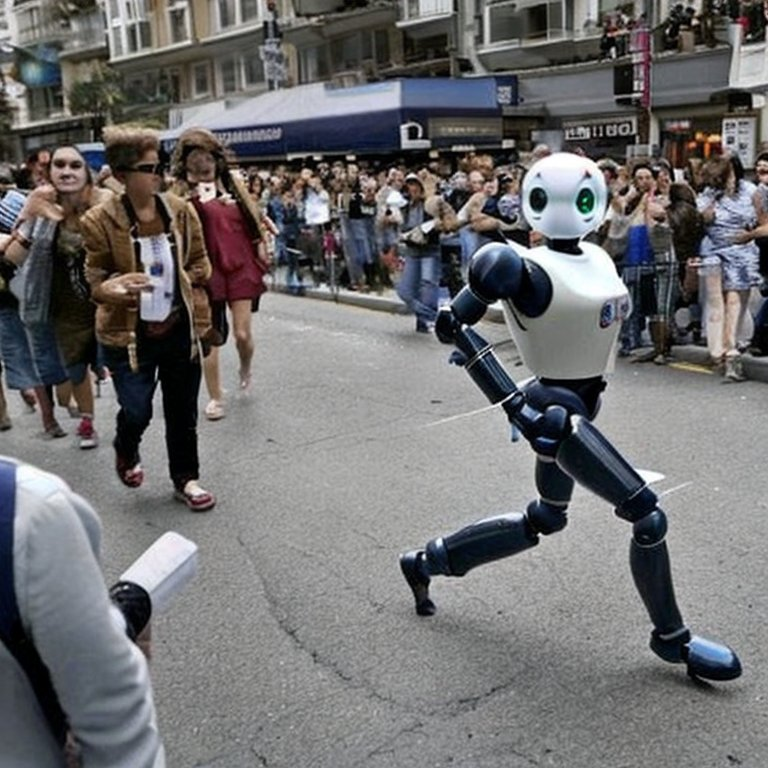
\includegraphics{robotmob}
        \caption{"a robot being chased by a mob of human onlookers Associated Press" made with Stable Diffusion 2.1}
        \labfig{robotmob}
\end{marginfigure}

One crucial aspect to consider when evaluating the practicality of Asimov's laws is the concept of consent. Human beings have the right to make decisions about their own safety and well-being, even if those decisions may carry risks. By strictly adhering to the First Law, AI systems may inadvertently undermine human autonomy and choice, leading to a paternalistic relationship between AI and its human users. It is essential that AI systems are designed to respect and prioritize human consent, ensuring that individual autonomy is preserved.

The Third Law, which requires a robot to protect its own existence, introduces an unnecessary and potentially problematic element of self-preservation. In the realm of AI and robotics, it is crucial that these systems have a built-in mechanism to shut down or be controlled when necessary. In this context, an "off button" serves as a vital safety measure, allowing human operators to intervene and regain control over a potentially malfunctioning or misaligned AI system.

Asimov's Third Law, by prioritizing the protection of a robot's existence, inadvertently creates the potential for conflict between the AI and its human operators. Security by obscurity can be a valuable approach to ensure that AI systems remain under human control, preventing the possibility of AI systems becoming dangerous or adversarial.

\section{You Can't Handle The Truth!}

Deep learning systems, which form the backbone of many AI applications, are notoriously difficult to interpret. As these systems become more complex and integrated into various aspects of our lives, the need for transparency and interpretability becomes increasingly crucial. The legal and ethical implications of AI actions can be challenging to navigate, particularly in high-stakes environments such as warfare \cite{saferalgorithmicsystems}.

Consider, for example, the difficulties faced in explaining a self-driving car's actions in court. The problem becomes even more daunting when trying to justify the decisions made by an autonomous weapon. Without a clear understanding of the underlying logic and decision-making processes, the consequences of AI-driven actions may lead to ethical dilemmas and questions of accountability.

Machine learning models are only as good as the data they are trained on. Biased training data can lead to biased outcomes, which can have far-reaching consequences, particularly in the context of autonomous weapons. Moreover, the nature of threats and warfare is constantly evolving. This concept drift makes it difficult for AI systems to adapt to new situations and can be exploited by adversaries to gain an advantage.

The dynamic and ever-changing landscape of warfare necessitates AI systems capable of learning and adapting in real-time. Failure to address the challenges posed by concept drift and biased training data can lead to suboptimal decision-making and the potential for unintended harm.

\begin{marginfigure}[-5.5cm]
        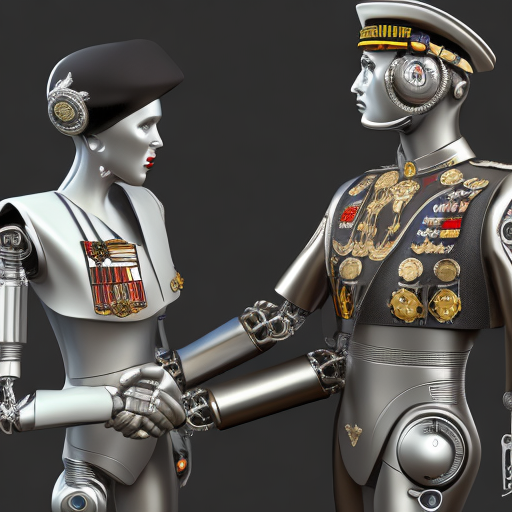
\includegraphics{sailor}
        \caption{"mdjrny-v4 style a robot wearing military medals, talking to a sailor 8k" made with Mann-E}
        \labfig{sailor}
\end{marginfigure}

AI systems, particularly those used in warfare, may be vulnerable to adversarial attacks. These attacks can exploit weaknesses in the AI's algorithms, causing the system to behave in unpredictable or undesirable ways. In some cases, adversarial attacks could even turn an AI system against its creators.

Imagine a scenario in which an adversarial nation-state discovers a weakness in an AI-powered reconnaissance drone. By exploiting this vulnerability, they are able to manipulate the drone's AI, causing it to transmit false intelligence or even engage in hostile actions against friendly forces. The consequences of such an event could be disastrous, undermining trust in AI systems and potentially escalating conflicts.

As we continue to develop and deploy AI-driven systems in the context of warfare, it is essential to address the challenges of interpretability, transparency, biased training data, and vulnerability to adversarial attacks. By doing so, we can ensure that AI serves as a force for good, enhancing our ability to protect and defend ourselves while minimizing the risks of unintended harm.

\section{AI Doesn't Kill People, People Kill People}

\textit{"First World War was known as 'the war to end all wars,' although some historians now argue it didn't. But it was the first high-tech war, with aeroplanes, machine guns and tanks all rising up to fight the human beings that made them. Despite having no beliefs or ideology or hearts or souls, the killing machines were victorious. The final score was weaponry 20 million, mankind nil."} Cunk On Earth Season 1 Espisode 3 \cite{cunkonearth}

The discourse surrounding AI in warfare often tends to be imprecise and misleading, resulting in a distorted understanding of the role artificial intelligence plays in modern conflict. AI-powered tools may indeed enhance military capabilities, but it is crucial to recognize that these weapons are AI-enabled, not autonomous. They operate under human command and control, serving as an extension of human decision-making rather than as independent actors \cite{aiwarfare}.

\begin{marginfigure}[-5.5cm]
        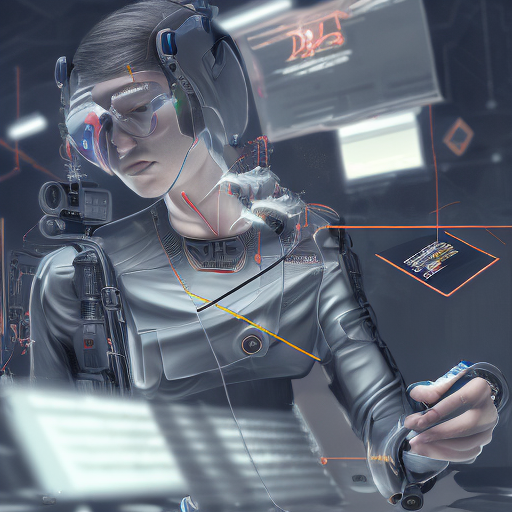
\includegraphics{droneop}
        \caption{"mdjrny-v4 style a human military drone operator using a joystick at his desk The Economist " made with Mann-E}
        \labfig{droneop}
\end{marginfigure}

To attribute blame or responsibility to AI in the context of warfare is to fundamentally misunderstand the nature of these systems. Artificial intelligence is a tool, one that can be wielded by human beings for various purposes, both benign and malicious. Just as a hammer can be used to build or destroy, AI can be employed to improve lives or inflict harm. The key determinant in each scenario is the intent and actions of the person wielding the tool, not the tool itself.

In our pursuit of technological advancements and AI-driven military capabilities, it is essential to maintain a clear and accurate understanding of the relationship between human actors and the tools they employ. By doing so, we can foster a more informed and nuanced conversation about the role of AI in warfare and the ethical implications that come with its use.

As we continue to develop and deploy AI-enabled weapons, let us never lose sight of the fact that it is ultimately people who make the decisions and bear the responsibility for their consequences. It is our collective responsibility to ensure that we use AI ethically, responsibly, and in the service of peace, rather than allowing it to become a mere instrument of destruction.

\section{Key Takeaways}

\begin{itemize}
\item \textbf{Autonomous weapons are not self-determined} AI-enabled weapons require human oversight and control, emphasizing that the responsibility for their use and consequences lies with human decision-makers.
\item \textbf{Intelligence does not equate to a drive for dominance} AI systems are tools designed to acquire and apply knowledge in pursuit of a goal, but the goal itself is determined by human actors, not the AI.
\item \textbf{Asimov's Third Law is flawed} AI systems need an off button and should not be designed to prioritize their own preservation over ethical considerations.
\item \textbf{Transparency and interpretability are crucial} The challenges of understanding AI systems' decision-making processes must be addressed to ensure accountability and ethical use in warfare.
\item \textbf{Address biases, concept drift, and adversarial attacks} Ensuring that AI-driven systems are robust, adaptable, and free of biases is essential for their responsible and effective deployment in the context of warfare.
\end{itemize}
